\chapter{Especificación y requisitos}

Pasemos ahora a describir de la forma más detallada posible cada uno de los requerimientos que conforman la idea del proyecto, planteando del mismo modo alternativas o aspectos que sería de agrado incluir, si bien no forman parte de la especificación inicialmente. Las decisiones tomadas, así como las soluciones implementadas, serán detalladas en el capítulo siguiente, si bien a lo largo de éste mismo pueden surgir necesidades cuya solución se detalle directamente.\\

Se desea disponer de una plataforma robótica extensible, libre y abierta; que permita una buena ampliación de nuevas características mediante software. Además, se propone la implementación de un uso concreto para esta plataforma, y es que dicho robot sirva como \textbf{guía de caminos} para sus usuarios finales en un \textbf{entorno controlado}. En este capítulo listaremos los distintos requisitos y puntualizaremos sobre cada una de las decisiones tomadas para satisfacerlos.\\

\section{Requisitos generales}

Los requerimientos aquí listados comprenderán cosas tanto de procedimientos para el desempeño del proyecto (como pueden ser la visibilidad y su legislación) hasta las funcionalidades más concretas que se esperan del producto final.\\

\subsection{Licencias}

Se tratará de un proyecto de software \textbf{libre} y de \textbf{código abierto}. Para ello, se publicará bajo una licencia \textit{GPLv3} en un repositorio público en \textit{Github}.\\

Además de \textit{Github}, existen otras alternativas de repositorios públicos que permiten utilizar \textit{git} para control de versiones (como \textit{Bitbucket} y \textit{Gitlab} entre otras). El porqué de utilizar \textit{Github} es meramente por aprovechar la licencia \textit{premium} que se provee a los estudiantes de la UGR simplemente por matricularse; permitiendo así tener algunos repositorios privados a su disposición \cite{github-premium}.\\

Con el código público y la licencia elegida, cualquier usuario podrá descargar el software, compilarlo, ejecutarlo e incluso añadir modificaciones al código para ser probadas e integradas en la plataforma final. Para ello, en el propio repositorio se pondrá a disposición de los interesados una documentación que explique cómo replicar el entorno tanto de desarrollo como de compilación.\\


\subsection{Especificaciones}

El término \textit{plataforma robótica} puede ser demasiado amplio para su manejo, por lo que en esta sección detallaremos más a fondo algunos de los puntos más interesantes, así como los factores de éxito que harían de \textbf{\textit{Lazarillo}} un producto útil y diferencial con respecto a las alternativas ya existentes.\\


\subsubsection{Extensibilidad}

Ya que se desea disponer de una plataforma extensible cuyo comportamiento y características puedan ampliarse a través de software, se debe dotar al robot de una arquitectura que permita este crecimiento, conteniendo en ella servicios (o módulos) independientes que puedan incluirse o no en función de la aplicación específica que vaya a cumplir el robot.\\

Para ello, sería interesante disponer de una arquitectura basada en \textbf{microservicios} donde cada uno de ellos cumple un propósito muy concreto y se comunica con el resto sin generar acoplamiento. Para esto es de imperativa necesidad utilizar un paradigma de comunicación en el cual sea transparente añadir datos y servicios.\\

Por otro lado, ha de asegurarse que existe la \textbf{interoperabilidad}, la cual representa que una arquitectura que incluye distintas plataformas de hardware y diferentes sistemas software (implementados con lenguajes de programación variados) cooperan bien entre sí.\\

Veamos un ejemplo rápido para ilustrar el párrafo anterior: si el programa que recibe los datos de un servidor web está programado en \textit{Python} y debe transmitirlos al servicio que toma las decisiones de movimiento (programado en \textit{C++}); el paradigma de comunicación que los conecta ha de ser \textbf{agnóstico en el lenguaje} y que dicha operación sea efectiva de forma transparente.\\


\subsubsection{Conectividad}

Como plataforma inteligente y conectada que utiliza el paradigma del \textbf{\textit{edge computing}}, sabemos que el robot ha de ser un dispositivo embebido con conexiones al exterior como \textit{Bluetooth} y/o \textit{WiFi}. Que éstas vengan implícitas en la plataforma hardware utilizada facilitará mucho el trabajo, ya que nos ahorramos el hecho de tener que soldar componentes. En cuanto a plataformas hardware, en el apartado del \textbf{Estado del Arte} ya comentamos algunas alternativas y opciones. Utilizaremos para ésto una \textit{Raspberry Pi Model 3 B}, que pese a no ser el último modelo de la marca \textit{Raspberry}, es la que tengo a disposición en casa. Además, satisface las necesidades de conectividad que comentábamos.\\

Por otro lado, en cuanto al requisito de computación en el borde, la plataforma deberá contener uno o más servicios que permitan la comunicación con el exterior, de una forma u otra, además de enviar y recibir mensajes. El robot deberá habilitar un canal de comunicación \textbf{persistente} y \textbf{bidireccional} que le permitan tanto a él como al servidor enviarse eventos entre sí.\\


\subsubsection{Interfaz y experiencia de usuario}

El robot contará con una pantalla táctil con la que proveerá la información necesaria al usuario (en función de las aplicaciones que necesite o decidan integrarse en el robot). Cualquier pantalla táctil que permita su conexión con la \textit{Raspberry} debería servir, por lo que no entraremos a detallar limitaciones hardware. Para la interacción del usuario, el sistema contará con una \textbf{aplicación embebida de entorno gráfico} que permita el uso del robot.\\

Dado que \textbf{\textit{Lazarillo}} se pretende que actúe como \textbf{guía}, otra característica que sería de agradecer en la plataforma tiene que ver con la \textbf{reproducción de sonidos} que faciliten la comunicación con el usuario, así como la \textbf{accesibilidad}. No todo el mundo goza de capacidad visual o simplemente no están habituados a interfaces táctiles, por lo que emitir alertas y sonidos descriptivos facilitaría llegar a más usuarios de forma plena y satisfactoria.\\

\subsubsection{Gestión experta y mantenimiento}

Como hemos comentado en secciones anteriores, el robot gozará de hardware provisto de conectividad inalámbrica. En este punto haremos uso de esta característica para ofrecer un método de mantenimiento, supervisión y gestión del robot, por parte de alguna "mano experta". Necesitaremos un método de administración de los distintos robots existentes desde un portal web externo a ellos. Un técnico encargado de gestionar los robots, accederá a una web alojada en un servidor a través del protocolo común de \textit{HTTP}.\\

Inicialmente, este portal web servirá para listar los dispositivos conectados (es decir, los robots que han sido provisionados con el software de \textit{Lazarillo} y se encuentran en funcionamiento), pero posteriormente permitirá enviar acciones remotas desde el servidor al robot (como reinicios, actualizaciones de software, acciones concretas a realizar por el robot, etc.).\\

Es deseable que la interfaz web sea sencilla y usable. Además, sería de agradecer que ésta pueda visualizarse correctamente en \textbf{dispositivos móviles}, ya que ampliaría el rango de posibilidades de gestión de los dispositivos robóticos.\\

\subsubsection{Movilidad}

El factor determinante que diferenciará a nuestro robot de un sistema empotrado inmóvil será la capacidad de desplazarse por el entorno. Ya sea para un uso u otro, el robot deberá venir dotado de un sistema hardware que le permita avanzar por el plano, conteniendo elementos como \textbf{motores} y \textbf{ruedas} o \textbf{cintas móviles}.\\

Además, si se desea que el robot sea \textbf{inteligente} y reconozca el entorno por el que se está moviendo, deberá dotarse de algún sistema de reconocimiento como \textbf{sensores de proximidad} o \textbf{cámaras}. Respecto a esto, si queremos seguir el paradigma de \textit{edge computing} como venimos comentando, el procesamiento de estas señales podría realizarse en el servidor en lugar de en el propio robot, lo que también liberaría a la plataforma hardware del robot de una buena parte de la computación.\\

Para acotar el alcance del proyecto y que sea asumible para un trabajo de este calibre, inicialmente la movilidad podrá estar basada en hacer \textbf{seguimiento de líneas} sobre el suelo.\\

\begin{figure}[h]
	\centering
	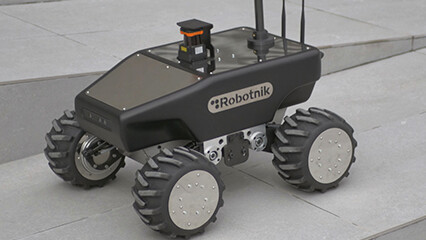
\includegraphics[width=0.6\textwidth]{imagenes/robotnik.jpg}
	\caption{Ejemplo de robot móvil autónomo - Fuente: \textit{Robotnik}}
\end{figure}


\section{Objetivos opcionales}

En esta sección enumeraremos y describiremos sucíntamente qué otras ideas surgieron durante el momento de \textit{brainstorming} del proyecto, y que si bien son opcionales para su desempeño, realmente aportarían algún valor al producto final.\\


\subsubsection{Movilidad autónoma}

Un factor que haría de \textbf{\textit{Lazarillo}} un producto totalmente independiente y útil sería que no necesitase de caminos guiados para desplazarse. Se valoraría la instalación en sí mismo de los mapas cerrados en que se ubicaría durante su desempeño, así como un mecanismo de \textbf{geolocalización} en el espacio. Contando con esto, el robot mantendría una comunicación persistente con el servidor informando en \textit{tiempo real} de la ubicación actual.\\





